% !TEX root = root.tex
\chapter{\label{chap:photoactivation}Multiscale Nanoparticle Mobility Measurements in Biological Gels Using Photoactivatable Fluorescent Probes}
\chaptermark{Photoactivation}

\section{Introduction}

Drug-delivery nanoparticles often must diffuse through biological barriers to achieve therapeutic efficacy at their target site. In some instances, such as tear film at the ocular surface, the barrier is only a few micrometers thick \cite{King-Smith2000,Azartash2011}. In other cases, nanoparticles must penetrate tens of micrometers or more through viscoelastic biological gels or tissue \cite{Nance2012,Xu2013,Schuster2013}. Measurements \emph{in vitro} at physiologically relevant length scales are valuable for designing nanoparticles that will exhibit favorable \emph{in vivo} biodistribution.
Here, we present a strategy for measuring nanoparticle mobility in biological gels over length scales ranging from sub-micrometer to tens of micrometers using photoactivatable fluorescent probes. This work is part of a collaboration with Benjamin Schuster and Joshua Kays in the laboratory of Professor Justin Hanes in the Center for Nanomedicine of JHU.

The study involved polymeric nanoparticles with a dense polyethylene glycol (PEG) coating to minimize particle adhesion to the gel. The particle core was imbued with photoactivatable (caged) rhodamine, which becomes fluorescent only if the rhodamine is ``uncaged'' through momentary exposure to UV light. This functionality permitted us to selectively photoactivate a region of particles with a brief pulse of UV light, and then observe the spread of the fluorescent particles in the gel over tens of micrometers and tens of minutes, all using confocal microscopy. Complementing these measurements, we were also able to quantify the motion of the photoactivated particles at high spatiotemporal resolution --- tens of nanometers and tens of milliseconds --- using multiple particle tracking (MPT) on a widefield microscope. MPT has been harnessed recently to measure transport of drug delivery nanoparticles in many biological materials, including brain tissue\cite{Nance2012}, mucus\cite{Lai2009,Wang2008,Schuster2013}, vitreous\cite{Xu2013}, and inside cells\cite{Crocker2007}. MPT is a powerful technique that permits examination of individual particles and analysis of heterogeneous transport behavior. However, because of the limited depth-of-field of high-numerical-aperture objectives, tracking particles diffusing in three dimensions for more than a few seconds and a few micrometers is difficult. The photoactivation method described here provides another approach to directly observe percolation through biological gels over longer distance and time scales. Hence, particle tracking and the photoactivation technique are complementary methods that, together, permit multiscale diffusion measurements. 

We first confirmed agreement between measurements from MPT and the photoactivation technique on particles diffusing in water. Then, we applied our method to fibrin, a model protein gel system, and found that both MPT and the photoactivation method reveal mobile and immobile populations of particles. Finally, we examined nanoparticle diffusion in sputum collected from cystic fibrosis (CF) patients. Sputum is a major barrier to inhaled CF therapeutics, and our approach enabled us to measure particle diffusion over distances relevant to drug delivery in the lungs, revealing large-scale heterogeneity in the mobility that might be missed with techniques surveying motion over shorter length scales.
\section{Experimental Methods}
\subsection{Materials}
Cholalic acid sodium salt (CHA), NVOC2-5-carboxy-Q-rhodamine-NHS ester (caged rhodamine-NHS ester), N-hydroxysulfosuccinimide sodium salt (sulfo-NHS), and N-(3-Dimethylaminopropyl)-N'-ethylcarbodiimide hydrochloride (EDC) were purchased from Sigma-Aldrich (St. Louis, MO). Poly(lactide-co-glycolide(75:25)) amine endcap (PLGA-NH2), Mn 10kDa-15kDa was purchased from Polyscitech (West Lafayette, IN). Poly(lactide-co-glycolide(67:33))-polyethylene glycol (45kDa-5kDa) diblock copolymer (PLGA-PEG) was custom-synthesized by Jinan Daigang Biomaterial Co., Ltd, (Jinan, China). 5 kDa methoxy-PEG-amine was purchased from Creative PEGWorks (Winston Salem, NC). Fluorescent carboxylate-modified polystyrene microspheres (PS-COOH) of diameter 100, 200, and 500 nm were purchased from Molecular Probes (Eugene, Oregon). Human $\alpha$-thrombin (activity 3059 NIH U/ml) and human fibrinogen (plasminogen depleted, activity 100\%) were purchased from Enzyme Research Laboratories (South Bend, IN).
\subsection{Particles}
The particles were designed and synthesized by my collaborators, Benjamin Schuster and Joshua Kays. Their protocol is presented here for context.
\subsubsection{Labeling of PLGA with caged rhodamine}
Caged rhodamine-NHS ester and PLGA-amine were conjugated through formation of an amide bond. Briefly, 90 mg of PLGA-NH2 was added to 5 mg of caged rhodamine-NHS ester (for a slight molar excess of dye compared to PLGA, 1:1.23) and put under vacuum for 1 h. The mixture was then flushed with nitrogen gas, dissolved in 500 \textmu l of anhydrous dichloromethane (DCM), and reacted for 12 h at room temperature under nitrogen gas. Additional DCM was added as needed to facilitate transfer of the product into 10 ml of -20 $^\circ$C diethyl ether to precipitate the product. The PLGA, now conjugated with rhodamine, was washed twice in cold ether by centrifugation. Excess ether was decanted off and the final product, the purified PLGA, was placed in a lyophilizer (FreeZone 4.5 Plus; Labconco) for 12 h. The dried PLGA was stored at  -20 �C  in a shielded container to prevent exposure to incident UV light.
\subsubsection{Particle formulation: PS-PEG} 
PEGylated polystrene (PS-PEG) particles were used a control in particle tracking experiments to verify that the mobility photoactivatable particles was the same as more widely used PS-PEG particles. PS-PEG particles were prepared as previously described\cite{Nance2012} by coupling PS-COOH with PEG-amine using carbodiimide chemistry1. Generally, 100 \textmu l of stock (2\% solids) PS-COOH particle solution was added to borate buffer (pH 8) with 4 fold molar excess 5k mPEG-amine, EDC, and sulfo-NHS. The particles were reacted for at least 2 h, then washed three times by centrifugation and stored in DI water at 4� C.
\subsubsection{Particle formulation: PLGA-PEG}
Photoactivatable PLGA/PLGA-PEG nanoparticles were prepared by using the emulsion method according to the literature\cite{Xu2013}. Briefly, a 40 mg mixture (19:1 by mass) of PLGA-b-PEG5k and PLGA-caged rhodamine was dissolved in 400 \textmu l of DCM, making a 100 mg/ml solution. This solution was injected into an ice-cooled 5 ml of 0.5\% CHA aqueous solution, and sonicated at 30\% amplitude for 2 min using a 130 Watt probe sonicator (Sonics \& Materials, Newtown, CT) to form an oil-in-water emulsion of the organic phase (polymer and DCM) into the aqueous phase, stabilized by the CHA surfactant. The emulsion was immediately added to 35 ml of 0.5\% CHA solution and stirred at 600 rpm for at least 3 h to allow for complete particle hardening. The final particle suspension was filtered through a 5 \textmu m and then 0.45 \textmu m syringe filter, then the particles were collected and washed three times via centrifugation at 20,000 g for 25 min. The particles are depicted in Figure \ref{fig:particles} in a TEM image and in suspension in water, demonstrating their photo activatable capability.

   \begin{figure}
    \centering
    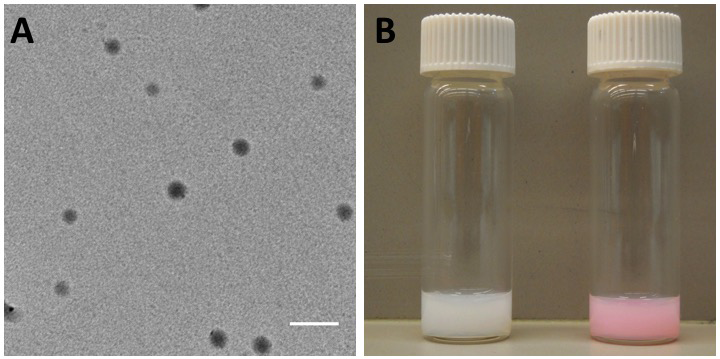
\includegraphics[width=\columnwidth]{photoactivation/particles}
    
    {\label{fig:particles}Panel A shows a TEM image of PLGA nanoparticles after dehydration. The white scale bar is 200 \textmu m. Panel B shows the particles in suspension in water before (left) and after (right) UV light exposure, demonstrating the activation of the caged rhodamine.}
    \end{figure}
    
\subsubsection{Particle Characterization}
The diameter and $\zeta$-potential of the nanoparticles were determined by dynamic light scattering and laser Doppler electrophoresis, respectively, using a Zetasizer Nano ZS90 (Malvern Instruments, Southborough, MA). Transmission Electron Microscopy (TEM) images of dried particles were taken on standard 400 mesh copper TEM grids (TedPella, Redding, CA) with a Hitachi H7600 Electron Microscope. Particles were 160 $\pm$ 10 nm in diameter with a PDI of 0.11 $\pm$ 0.02 and a $\zeta$-potential of -3 $\pm$ 1 mV, where error bars report variation between batches.

\subsection{Sample Preparation}
\subsubsection{Fibrin gel}
Human fibrin gel was made from defrosted aliquots of thrombin and fibrinogen. Appropriate particle concentrations (between 0.005-0.00004\% by mass) for tracking PS-PEG or PLGA-PEG particles were made in 2 U/ml thrombin in PBS, with a total volume of 180 \textmu l. 20 \textmu l of 40 mg/ml fibrinogen was pipetted to the solution, yielding a 4 mg/ml concentration of fibrinogen\cite{Spero2011}. Vortex was immediately applied at high speed for ~2 s to homogenize the solution. 30 \textmu l of the solution was immediately pipetted into a 30 \textmu l well on a glass slide, covered with a glass coverslip, and sealed with a cyanoacrylate glue. The slide was then incubated at 37 �C for 20 min to ensure gelation. In all cases, slides were wrapped in aluminum foil to prevent premature exposure to UV light. 
\subsubsection{CF Sputum}
CFS was collected from adult patients at the Johns Hopkins Cystic Fibrosis Center in accordance with Institutional Review Board-approved protocols. Samples were stored at 4$^\circ$C immediately after collection, and were analyzed the next day. CFS slides were made according to a similar procedure as the above for fibrin gels: 30 \textmu l aliquots of CFS were withdrawn using a Wiretrol (Drummond Scientific Company, Broomall, PA) and injected into 30 \textmu l wells on glass slides. 1 \textmu l of appropriate particle suspensions for tracking or for photoactivation was added to the aliquot and mixed thoroughly. The slide was then sealed and allowed to incubate at room temperature for 1-2 hours (to prevent convection effects).  

\subsection{Measurements}           
\subsubsection{Multiple Particle Tracking (MPT)}
Particle motion in the CF sputum and fibrin samples was observed at room temperature using an inverted epifluorescence microscope (Axio Observer; Carl Zeiss, Thornwood, NY) with a 100X/1.46 NA oil-immersion objective. Movies were collected with 19-ms exposure at 20 fps for 500 frames using an EMCCD camera (Evolve 512; Photometrics, Tucson, AZ). Particle motion was tracked using the particle-tracking software described in Chapter \ref{chap:trackpy}.

\subsubsection{Confocal imaging and photoactivation}
Confocal imaging was performed on a Zeiss LSM510 laser scanning confocal microscope (Carl Zeiss, Thornwood, NY) in multi-tracking mode using either the 63x (Plan Apochromat 1.4 NA), 40x (PlanNeofluar 1.3 NA), or 20x (Plan Apochromat .75 NA) oil-immersion objective. Particles in the selected regions were activated by 10 to 25 iterations of the 405-nm laser at 100\% power, while particles were excited to fluorescence by the 543-nm laser at 10--30\%  power.   All videos were $512\times512$ pixels, and the activated region was $40\times512$ pixels. (For experiments performed using 20X, 40X and 63X objectives, this corresponds to $35\times449$, $18\times225$, or $11\times143$ \textmu m$^2$, respectively.)
Slide preparation for confocal experiments was identical to the above procedure for multiple particle tracking in CFS, with the exception of particle concentrations: PLGA-PEG particles were added to either water, CFS, or fibrin with final concentrations of 0.075\% to 0.03\% by mass. 


\section{Results}

\subsection{Water}

Here we obtain the particles' diffusivity $D$ in water from the evolution of the observed fluorescence intensity $I(x, y, t)$ from photoactivated particles. To begin, we will take the system to be homogenous, an assumption which of course holds for water, but which we must revisit when addressing more complex systems in later sections. Figure \ref{fig:water}(a) displays a series of fluorescence images at different times following UV exposure to a strip-shaped region of the sample indicated by the red lines in the top image. We take the $y$-direction to be parallel to the strip and the $x$-direction to be perpendicular to it. The experiment is symmetric along $y$, and so the full image $I(x, y, t)$ can be summarized by an intensity profile $I(x, t) = \sum_y I(x, y, t)$. Under carefully tuned experimental conditions, intensity is directly proportional to the concentration of activated particles $c(x, t)$. Of course, this approximation is not universally applicable: particles overlap and scatter incident light and the emitted light from the particles around them, so at high concentrations the observed intensity must ultimately saturate. Also, the sensor imposes a sharp limit of the range of observable intensities. A carefully designed experiment, then, must match the particle concentration $c$ and fluorescence (controlled in part by the intensity of incident light) to the sensitivity of camera. In our experiments, departures from the linear approximation $I \propto c$ were measurable but small, less than 5\%.

In a viscous liquid such as water, the concentration profile evolves according to the diffusion equation:

\begin{equation}
 \frac{\partial c}{\partial t} = D\frac{\partial^2 c}{\partial x^2}
\end{equation}

\noindent An idealized, infinitely thin activation region at $x'$ and time $t'$, described by $c(x) = \delta(x-x')$, would evolve as a Gaussian that spreads during some time interval $t-t'$ as

\begin{equation}
 c(x, t) = \frac{1}{\sqrt{4\pi D (t-t')}}\exp\left[-(x-x')^2/4D(t - t')\right]
\end{equation}

\noindent This Gaussian is the Green function $G(x - x'; t - t')$ for the diffusion equation. Therefore, for any distribution of activated particles $c(x', t')$ at time $t'$, the distribution at some later time $t$ will be

\begin{equation}
 \label{eqn:convolution}
 c(x, t) = \int_{-\infty}^\infty G(x - x'; t - t')\, c(x', t')\,dx'
\end{equation}

\noindent and therefore, if $I \propto c$,

\begin{equation}
 \label{eqn:convolution}
 I(x, t) = \int_{-\infty}^\infty G(x - x'; t - t')\, I(x', t')\,dx'.
\end{equation}

\noindent That is, the intensity profile at $t'$ can be mapped onto the intensity profile at $t$ through convolution with a Gaussian with width $\sigma=\sqrt{2D(t-t')}$. Breakdown of this mapping would indicate non-diffusive motion, which is not expected for water but could occur in other materials.

   \begin{figure}
    \centering
    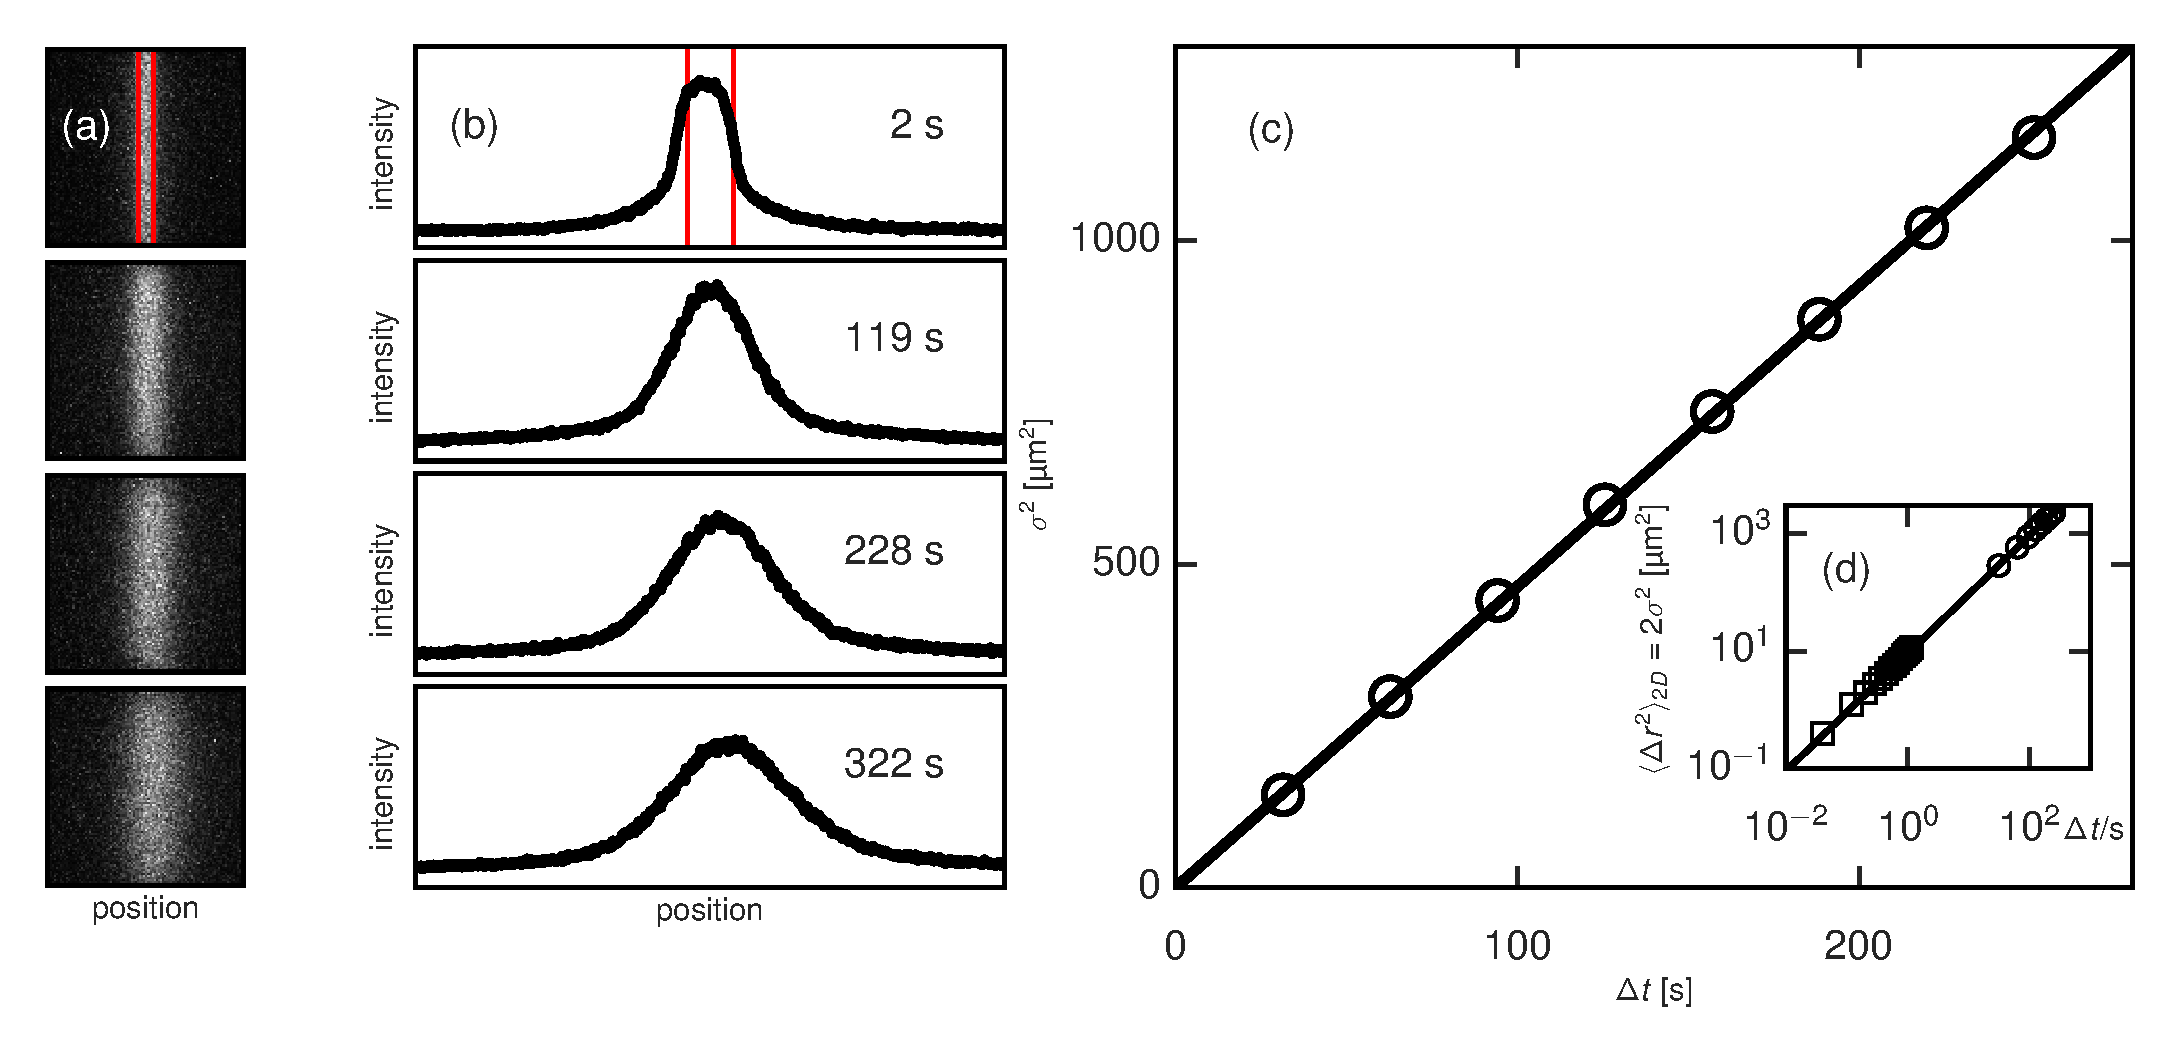
\includegraphics[width=\columnwidth]{photoactivation/water}
    \caption[Photactivatable nanoparticles diffuse in water. From the profile of intensity, diffusivity is extracted.]{\label{fig:water}Photactivatable nanoparticles diffuse in water. (a) The region outlined in red, which is 34 microns wide, is momentarily exposed to UV laser light, and any particles within that region become fluorescent. (b) Their subsequent diffusion is characterized by an intensity profile representing the summed intensity of each individual column in the image. Profiles at different times can be mapped onto each other through convolution with a Gaussian, as described in the text. (c) The Gaussian that maps a given profile at any $t'$ onto the profile at $t' + t$ has width $\sigma(t)$. This is related to the nanoparticles' diffusivity $D$ through $\sigma^2 = 2Dt$. We extract the value $D$=2.4 $\pm$ 0.1 \textmu m$^2$/s, which is within 5\% of the theoretical diffusivity of 170-nm particles in water at room temperature. (d) The particles were also studied using traditional multiple-particle-tracking (MPT), where all particles were activated and individually tracked in two dimensions. The mean-squared displacement of their trajectories $\langle \Delta r^2 \rangle_{2D}$ (squares) is shown alongside the Gaussian widths from (c), plotted once again as circles. The diffusivity obtained from MPT was $D$=2.421 \textmu m$^2$/s, in excellent agreement with the value obtained from photoactivation.}
    \end{figure}

During an experiment, hundreds of intensity profiles were captured at a regular interval. Every profile was mapped onto each future profile through convolution with a Gaussian, as in Eq. (\ref{eqn:convolution}). The width $\sigma$ of the Gaussian generating the most accurate mapping was determined using a nonlinear least-squares fit. Each mapping constituted a separate---though not strictly statistically independent---measurement of diffusivity $D$. Mappings corresponding to the same time interval $\Delta t = t - t'$ were averaged to produce the data points $\sigma^2(\Delta t)$ shown in Figure \ref{fig:water}(c). Finally, an estimate of $D$ was obtained through a linear regression to $\sigma^2(\Delta t)$. Its value, 2.4 $\pm$ 0.1 \textmu m$^2$/s, is within 5\% of the expected value for the diffusivity of 170-\textmu m particles in water, thus demonstrating the utility of the photoactivation approach as a microrheology technique. Figure \ref{fig:water}(d) shows the values of $\sigma^2$ from the photoactivation measurement along with those from MPT measurements. The two sets of results are consistent, and the figure indicates the complementary range of length and time scales each covers.

\subsection{Fibrin}

In experiments performed on samples of fibrin gel, some of the photoactivated nanoparticles spread with time outward from the activation region, but others remained immobilized, as evidenced by the still-bright activation region in Figure \ref{fig:fibrin-final-frame}, which depicts the intensity 785 seconds after photoactivation. The mobile and immobile populations can separated by comparing the full intensity profile $I(x, t=785\text{ s})$ to a Gaussian fit, where the fit is restricted to values of $x$ outside the initial activation region and extrapolated to within the activation region (Figure \ref{fig:fibrin-gaussian-portion}). Comparing the integrated area of the Gaussian to the excess intensity in the activation region, we estimate that the mobile particles make up 40\% of the total population. This fraction is compatible with our finding from MPT experiments in fibrin, which also show an approximately even split between mobile particles moving diffusively, $\langle \Delta r^2(t)\rangle \propto t$, and immobile particles characterized by a finite asymptotic MSD, $\langle \Delta r^2(t\rightarrow\infty)\rangle = \langle \Delta r^2 \rangle_0$. The MSDs of individual particles in fibrin derived from particle tracking are plotted in Figure \ref{fig:fibrin-msd}, illustrating this division of mobility into two populations. A histogram of $\langle \Delta r^2(t=1\text{ s})$, emphasizing the bimodal distribution of mobilities is shown in Figure \ref{fig:fibrin-msd-hist}.

We speculate that this bimodal distribution is a consequence of mesoscale heterogeneity in the fibrin gel that forms as a result of microphase separation during the gelation process. As the fibrogen polymerizes, the polymer solution undergoes spinodal decomposition. The phase separation is arrested, however, by the cross linking that locks in a bicontinuous structure of high and lower concentration gel. The porosity of the high-concentration regions is smaller than the particles, such that the particles are trapped in the gel. The fluorescence images directly capture this microstructure of the fibrin gel---the underlying spatial distribution of a polymer-rich phase, containing entrained particles, and a polymer-poor phase, which is essentially a viscous liquid in which the particles freely diffuse. The apparent length scale of this micro-scale phase separation, visible in Figure \ref{fig:fibrin-final-frame}, is about 10 \textmu m, which is less than the typical linear spacing between particles in the MPT experiments. This result thereby illustrates another way in which photoactivation complements MPT: the higher particle densities in photoactivation experiments resolve underlying structural heterogeneity that gives rise to the dynamic heterogeneity in the MPT experiments. (MPT experiments cannot be performed at such high particle densities due to both experimental and fundamental limitations discussed in Chapter \ref{chap:methods}.)

   \begin{figure}
    \centering
    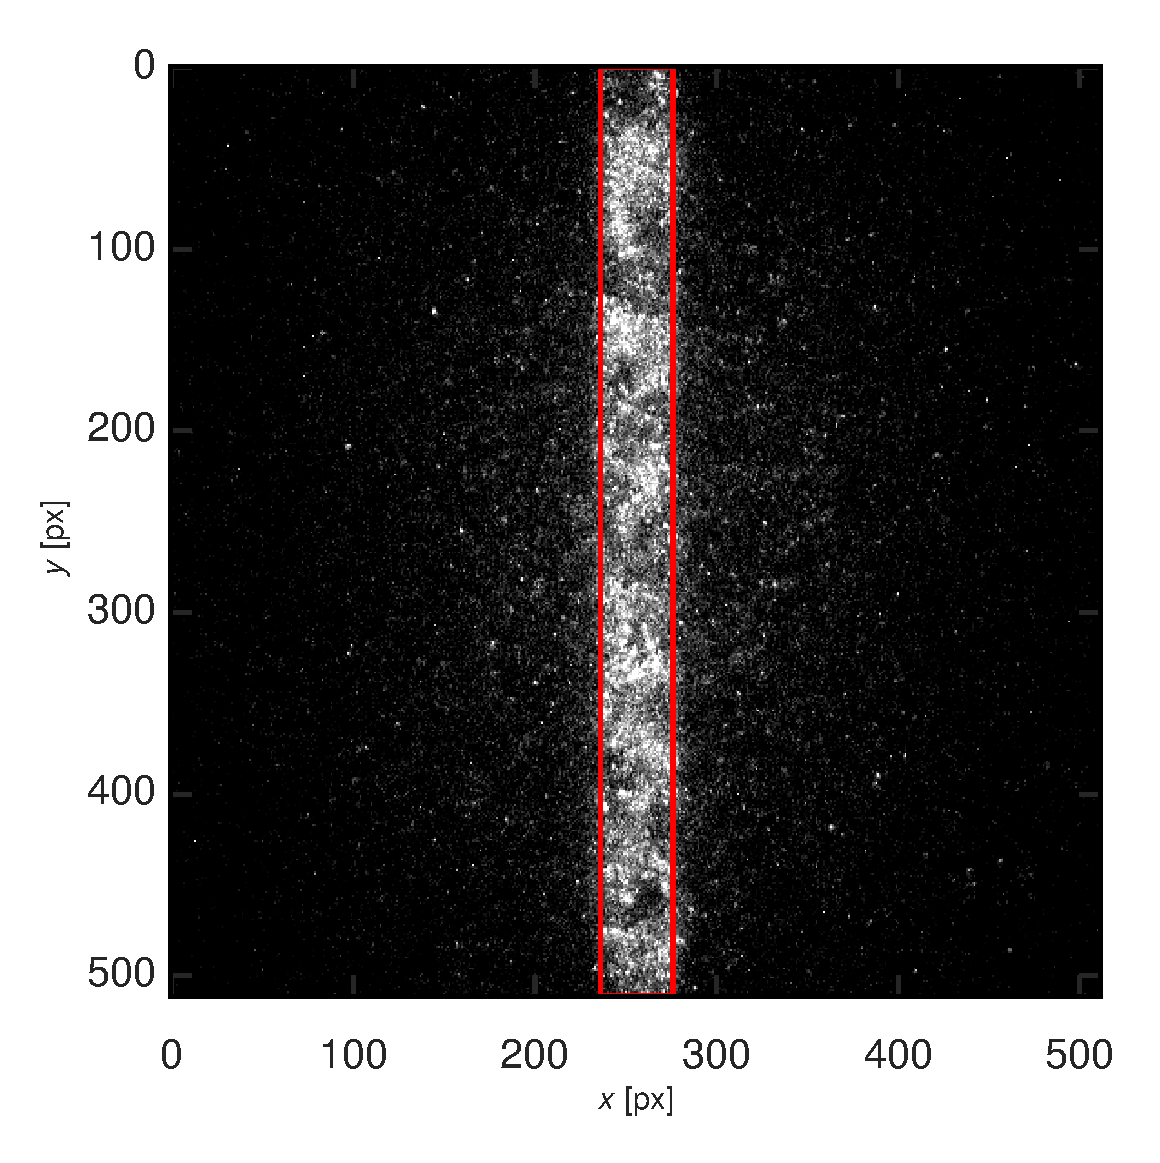
\includegraphics[width=\columnwidth]{photoactivation/fibrin-final-frame}
    \caption[Fluorescence intensity from photoactivated nanoparticles in fibrin 785 seconds after those in the activation region were activated with UV light.]{\label{fig:fibrin-final-frame}Fluorescence intensity from photoactivated nanoparticles in fibrin 785 seconds after those in the activation region (outlined in red) were activated with UV light. While some have spread outward as in Figure \ref{fig:water}, the lingering intensity in the activation region shows that others remain immobilized in the immediate neighborhood of their initial position.}
    \end{figure}
    
   \begin{figure}
    \centering
    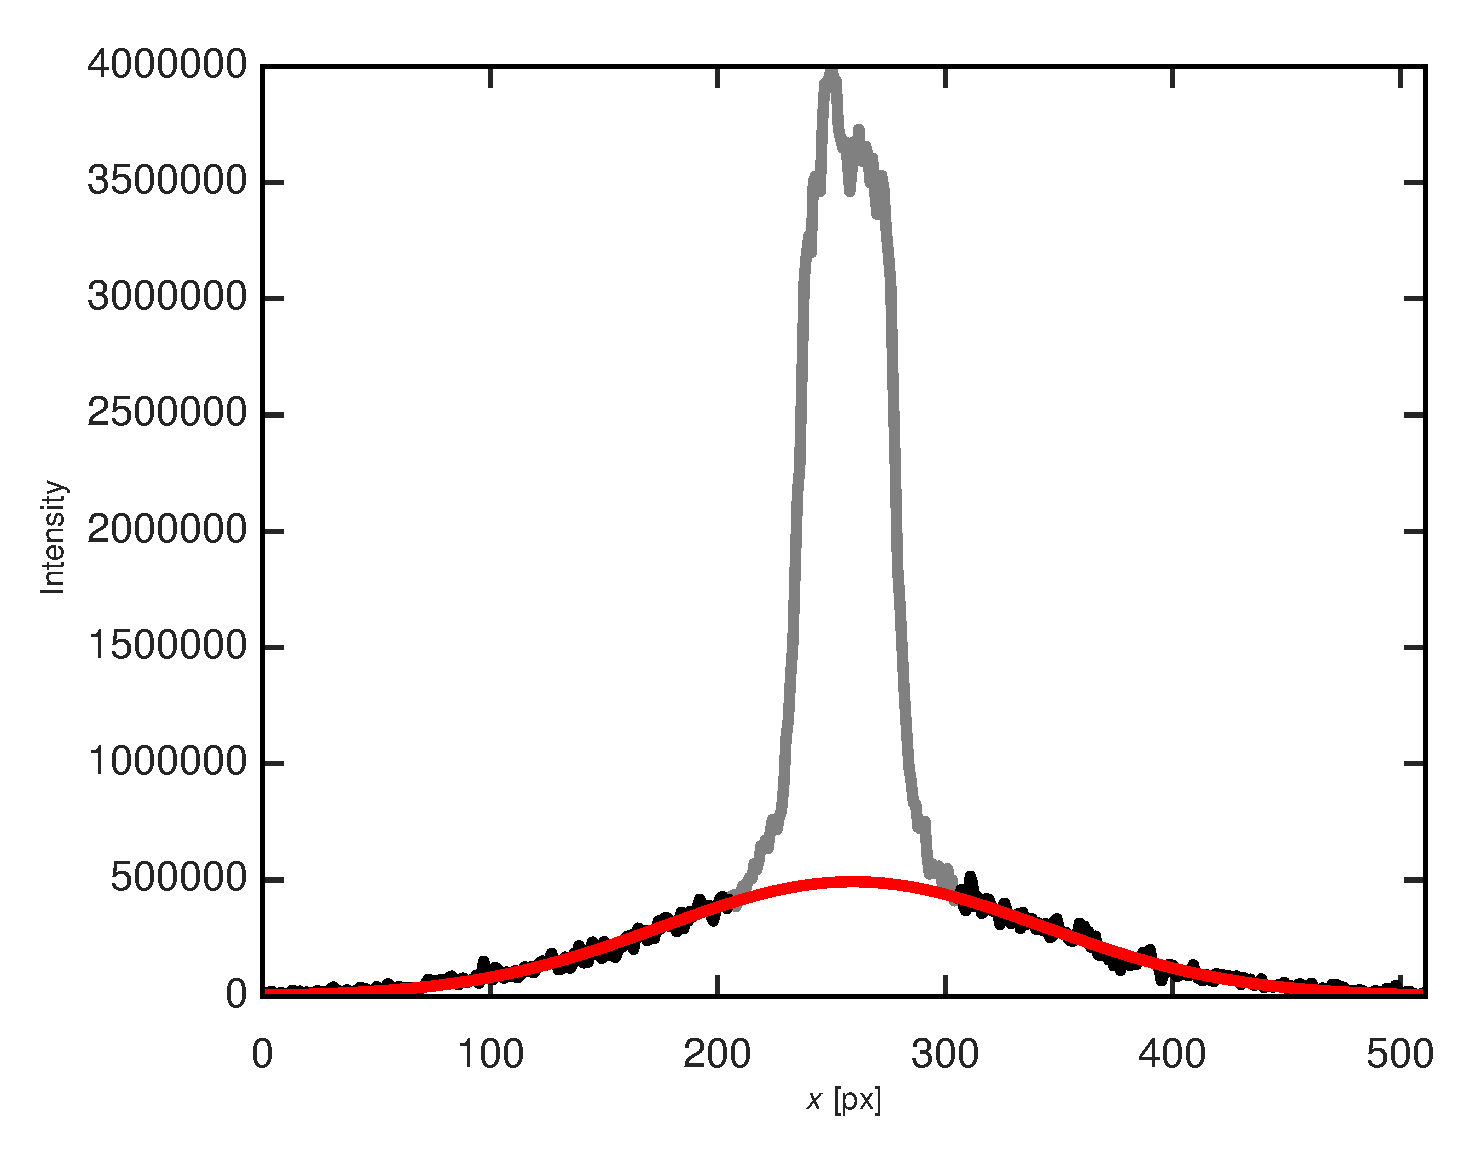
\includegraphics[width=\columnwidth]{photoactivation/fibrin-gaussian-portion}
    \caption[The intensity profile of photoactivated nanoparticles in fibrin, separated in mobile and immobile populations.]{\label{fig:fibrin-gaussian-portion}The gray-and-black curve shows the intensity profile $I(x, t)$ at t=785 seconds. In red is a Gaussian, fit only to the black portion of $I$ outside the initial activation region. We posit that the intensity under the Gaussian is due to mobile particles that happen to be diffusing in that region while the intensity over the Gaussian is due to immobilized particles that are not diffusing.}
    \end{figure}
    
       \begin{figure}
    \centering
    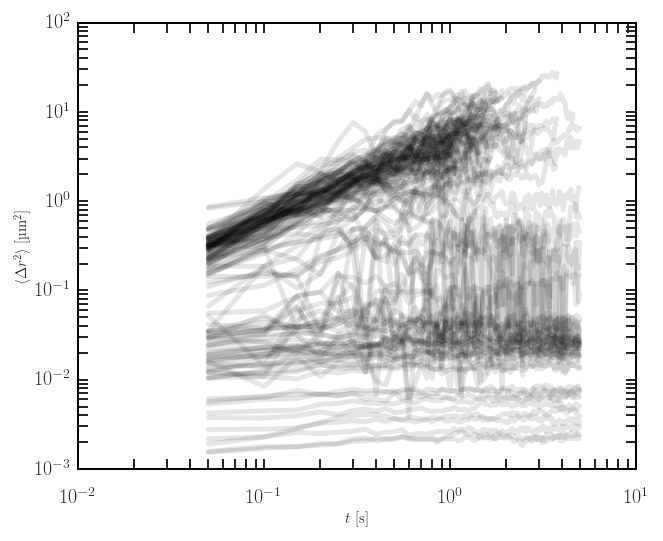
\includegraphics[width=\columnwidth]{photoactivation/fibrin-msd}    \caption{\label{fig:fibrin-msd}The MSD of individual PLGA-PEG particles in fibrin shows some particles moving diffusively and others jostling in place with an asymptotic MSD.}
    \end{figure}
    
           \begin{figure}
    \centering
    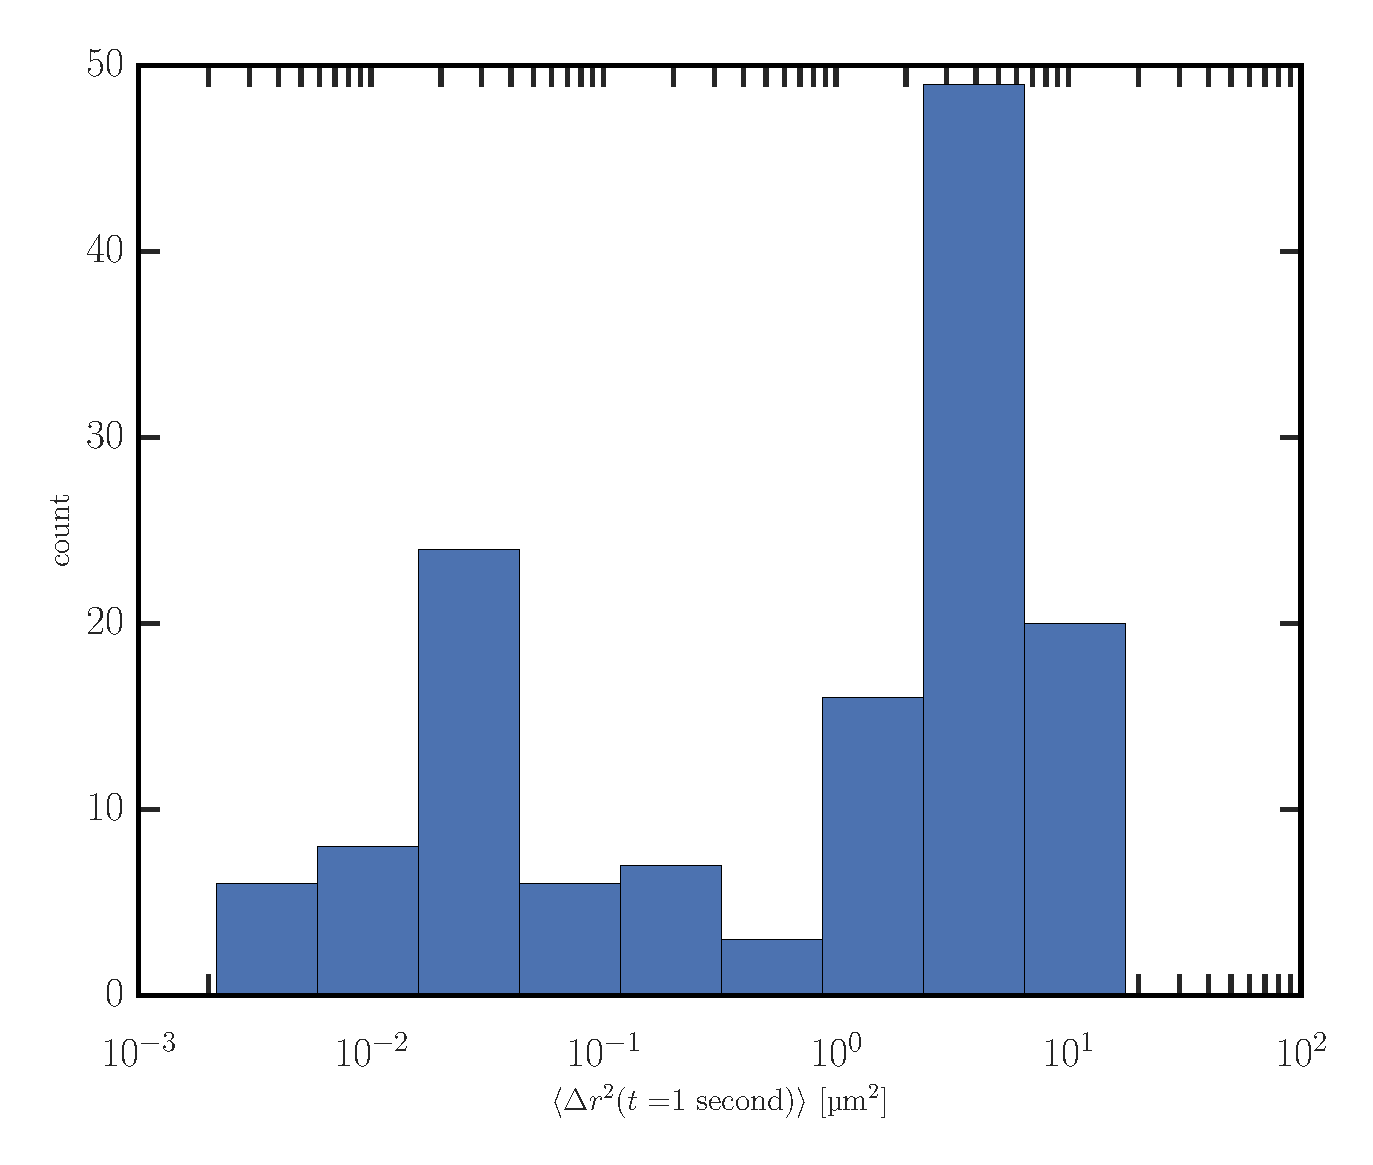
\includegraphics[width=\columnwidth]{photoactivation/fibrin-msd-hist}    \caption{\label{fig:fibrin-msd-hist}A histogram of the particles' MSD at lag time $t=$ 1 second shows an approximately equal division between mobile and immobile populations.}
    \end{figure}


\subsection{Cystic Fibrosis Sputum}

In particle-tracking studies, nanoparticles have been seen to diffuse through cystic fibrosis sputum (CFS)\cite{Schuster2013,Wang2008} over several micrometers, but in a CF patient the mucus barrier can be 20--50 \textmu m thick, or more, so it is important to show that nanoparticles can actually traverse tens of microns, the distance necessary to deliver therapeutic nanoparticles to lung cells. Heterogeneity in CFS has been seen in these particle-tracking studies, and it is unknown what impact this heterogeneity has on the long-distance mobility of nanoparticles in the sputum.

In addition to heterogeneity within a sputum sample, there is also patient-to-patient variation, which has been found to be the larger of these two effects\cite{SchusterThesis}. Characterization of nanoparticle mobility must contend with these variations. In our study, samples from one patient were found to be spatially homogeneous and approximately Newtonian. Thus, they were amenable to the same analysis performed on water above, as shown in Figure \ref{fig:simple-cfs}. From this analysis, we extract the diffusion coefficient $D=0.3994$ \textmu m$^2$/s, about an order of magnitude smaller than that in water.

   \begin{figure}
    \centering
    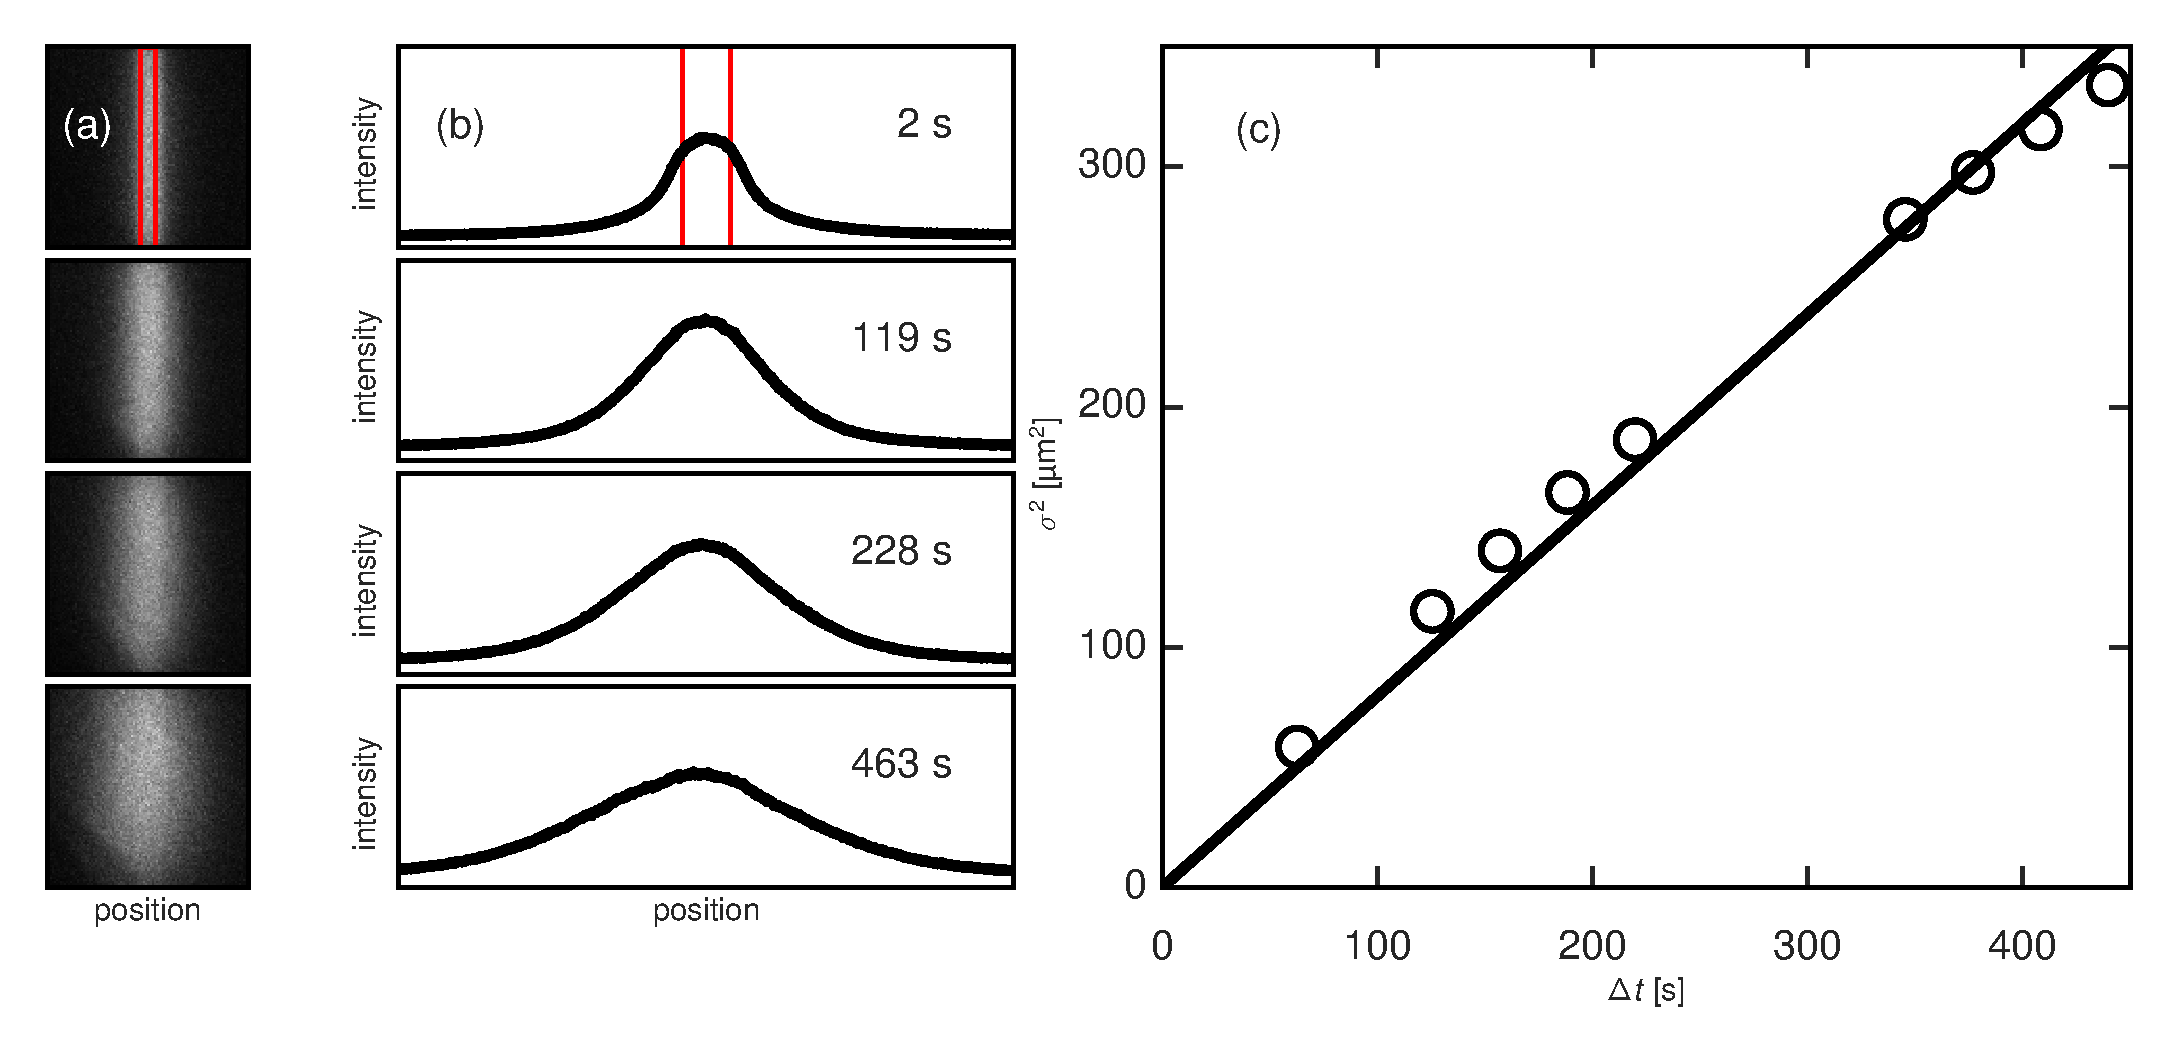
\includegraphics[width=\columnwidth]{photoactivation/simple-cfs}
    \caption[Photactivatable nanoparticles diffuse in sputum collected from a human cystic fibrosis patient.]{\label{fig:simple-cfs}Photactivatable nanoparticles diffuse in sputum collected from a human cystic fibrosis patient. As in Figure \ref{fig:water}: (a) The region outlined in red, which is 34 microns wide, is momentarily exposed to UV laser light, and any particles within that region become fluorescent. (b) Their subsequent diffusion is characterized by an intensity profile representing the summed intensity of each individual column in the image. Profiles at different times can be mapped onto each other through convolution with a Gaussian, as described in the text. (c) The Gaussian that maps a given profile at any $t'$ onto the profile at $t' + t$ has width $\sigma(t)$. This is related to the nanoparticles' diffusivity $D$ through $\sigma^2 = 2Dt$. We extract the value $D=0.3944$ \textmu m$^2$/s. (Missing data points are due to technical problems with video capture that, unfortunately, intermittently affected this particularly interesting trial.)}
    \end{figure}

Nanoparticle motion in samples from other patients was more complex and less amenable to straightforward application of such analysis. We observed mesoscale spatial heterogeneity, breaking the $y$-symmetry of the system, wherein the spreading particles made greater progress in certain subregions of the field of view. Illustrative examples are shown in Figure \ref{fig:cfs-gallery}. On a basic level, we see that nanoparticles can traverse tens of micrometers, so from a practical point of view this shows that it is possible for a PEG-coated nanoparticles to traverse CF sputum over a distance necessary to deliver therapeutic nanoparticles. To our knowledge, this is a new result. Of course, from the uneven permeability observed in Figure \ref{fig:cfs-gallery}, that delivery seems likely to be uneven across regions of the lung. Further, as with fibrin, photoactivation reveals the underlying microstructure of permeability that is difficult to discern from MPT analysis.

   \begin{figure}
    \centering
    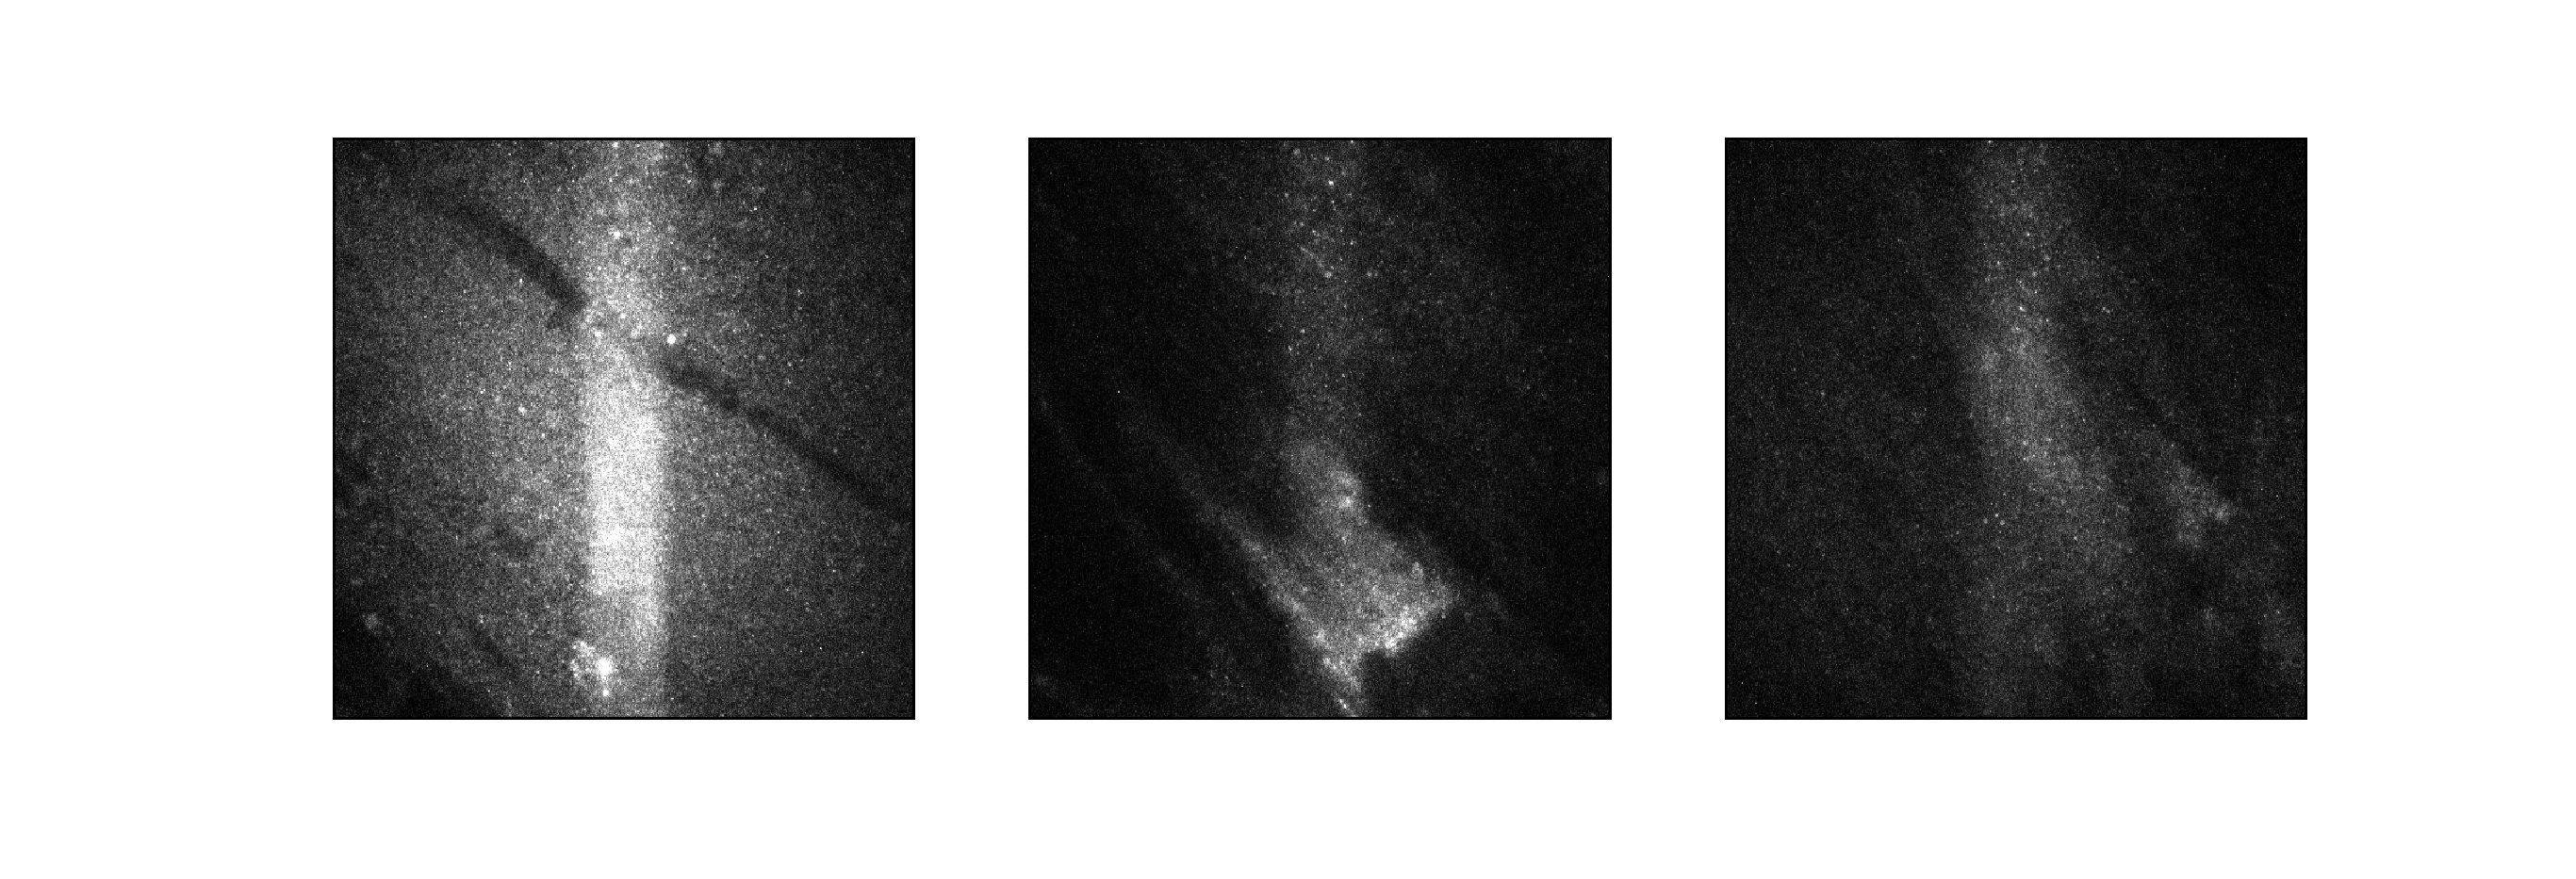
\includegraphics[width=\columnwidth]{photoactivation/cfs-gallery}
    \caption[In samples from some patients, dramatic heterogeneity was observed.]{\label{fig:cfs-gallery}In samples from some patients, dramatic heterogeneity was observed. These images depect the fluorescence intensity of photoactivated nanoparticles in three different samples from the same patient. At left, long substructures in the fluid are not permeated by the nanoparticles. At center, the particles spread more easily in the region at the lower-right part of the frame. At right, both of these kinds of effects are evident. The left and right images are taken 600 seconds (10 minutes) after activation; the center, 1570 s.}
    \end{figure}

\section{Discussion \& Conclusion}

We have developed a strategy of combining MPT with photoactivation for measuring nanoparticle diffusion in biological gels over multiple scales, ranging in time from tens of milliseconds to tens of minutes, and ranging in length from less than one micrometer to hundreds of micrometers.

The two techniques offer complimentary strengths. Particle tracking permits analysis of individual particles, and at high spatial and temporal resolutions, but the time and length of observation are limited. The photoactivation technique can monitor diffusion over longer times and distances, which are relevant in many drug-delivery applications, although spatial and temporal resolutions are not as good. Importantly, particle-tracking suffers from a sampling bias toward immobile particles, which stay in view longer and thus make up a disproportionate fraction of trackable particles\cite{Crocker2007}. The photoactivation technique, taking a wider view, captures the leading edge of diffusion and does not suffer from that particular bias.

In water, results from particle tracking and the photoactivation technique agree quantitatively. In fibrin, the two techniques portray compatible pictures of heterogeneous nanoparticle mobility. Finally, we directly observed PEG-coated PLGA nanoparticles diffusing over physiological distances in CFS and quantitified their diffusivity for one particular case that was unusually amenable to straightforward analysis. These findings extend prior, related work from the Hanes lab\cite{Schuster2013}.